\section{问题分析与求解思路}
\label{sec:overall_strategy}

\subsection{问题分析}

\subsubsection{问题一}

问题一包含“质量评价”和“领域配比响应”两条相互关联但统计单位不同的任务。质量侧以文档为单位，$22$ 项信号兼有标量、分类 logits 和结构统计量，不仅量纲与优劣方向不同，长度、数字比例等指标还可能存在适中区间；同时，多个质量维度可能对同一文本给出相反判断。为此，先对指标进行标量化、稳健同向化和语义分块，再采用稳定 CRITIC 权重与冲突自适应 Huber 聚合得到样本质量，并通过领域内 bootstrap 形成领域质量及其区间。

配比侧以训练配方为单位，$17$ 个领域份额满足非负且总和为 $1$ 的单纯形约束，不能把各份额当作彼此独立的普通自变量。本文采用二阶 Scheff\'e--Ridge 多输出混料模型拟合配比到 $13$ 个验证域 Loss 的响应面，以保持闭合的局部替换解释单域边际作用和两域交互；再利用 $1\mathrm{M}$、$60\mathrm{M}$ 和 $1\mathrm{B}$ 实测配方进行跨尺度检验，并在训练支持域内搜索带 bootstrap 区间的参考近优配比。

\subsubsection{问题二}

问题二需要把参数规模、训练数据量、数据质量和领域配比接入统一的 Loss 模型，但附件中不存在同时改变四类因素的联合实验，且 A、B 两组数据的模型族、验证集和响应尺度不同。若直接拼接观测，数据来源差异会与真实资源效应混杂。为保证可识别性，首先利用 B1 比较参数--数据可分幂律、总计算量幂律和交互幂律，通过留一规模验证确定经典标度律；随后在固定 $(N,D)$ 的 B7 质量网格上比较质量修正形式，以分组留出误差和简约性选择质量模型。

问题一的领域质量、参考配比和标准化配比响应只作为冻结接口输入，不直接充当 B 组绝对 Loss。本文以固定参考配比的广义标度律作为主模型，并将配比迁移强度作为需通过排序一致性、bootstrap 稳定性和不可约损失下界检验的扩展项。模型确定后，分别计算参数、Token 与质量的局部弹性和有限等 Loss 等价量，再用跨模型族数据、公开记录及压力测试数据界定外部有效性和外推范围。

\subsubsection{问题三}

问题三以问题二通过验收的广义标度律为目标函数，将基础训练成本 $6ND$、质量提升成本和长上下文注意力成本 $\eta NDL_{\mathrm{ctx}}$ 置于同一预算约束下。由于现有证据不足以识别配比强度与规模、质量之间的联合变化，主模型固定 $\boldsymbol p=\boldsymbol p_{\mathrm{ref}}$，只优化 $N,D,Q_A$，再按 $D_i=p_{\mathrm{ref},i}D$ 给出 $17$ 个领域的 Token 配置。预算 $C$、上下文长度和三类质量成本函数作为外生情景分别比较。

固定 $(N,Q_A)$ 时 Loss 随 $D$ 单调下降，因此可由预算等式解析消去 $D$，把三维问题化为二维有界优化。本文采用多起点求解、连续预算追踪和原始三维复核排除局部最优，并用 KKT 边际条件、成本份额与配置弹性识别质量投入启动、饱和等结构转移。最后通过联合 bootstrap、参数扰动和严格/扩展支持域标记，区分观测范围内的稳定结论与回答高预算情景所需的条件外推。

\subsubsection{问题四}

问题四需要从预训练 Loss 转向下游综合能力，并分离规模扩张与架构、数据工程、优化及后训练等非规模因素。附件 C 的排行榜、算力记录和 Loss--Benchmark 配对在评测协议、开放口径与时间覆盖上并不一致，若直接合并既会重复计数，也可能把桥接预测误当作历史观测。为此，先对多任务得分进行方向统一、缺失处理和同口径聚合，形成综合能力；再依据可比等级加权拟合有界单调的 Loss--Benchmark 桥接，并通过来源族留一验证确定映射形式及支持区间。

历史前沿只使用截止时点以前、开放权重且算力证据可追溯的模型记录，问题三的映射结果不反灌训练。本文以训练算力和时间状态刻画条件分位能力前沿，采用两因素 Shapley 路径平均分解首末时点变化中的规模相关贡献与非规模残余；随后从近期算力趋势构造增长延续及放缓情景，预测未来 $12$、$24$ 个月的能力前沿。模型族簇与月份块 bootstrap 用于同时传播桥接、前沿拟合和算力增长的不确定性。

\subsection{总体求解思路}

四问按照“数据属性--模型损失--资源决策--能力前沿”逐层推进。问题一输出质量基线、参考配比和配比响应；问题二将可识别的数据属性纳入广义标度律；问题三在通过验收的冻结接口上求解算力约束下的最优配置；问题四再把最优 Loss 映射到能力尺度，用于历史贡献分解与未来情景预测。整体的数据来源、模型接口、关键输出和验证关系如图~\ref{fig:overall_dependency}所示。

\begin{figure}[htbp]
\centering
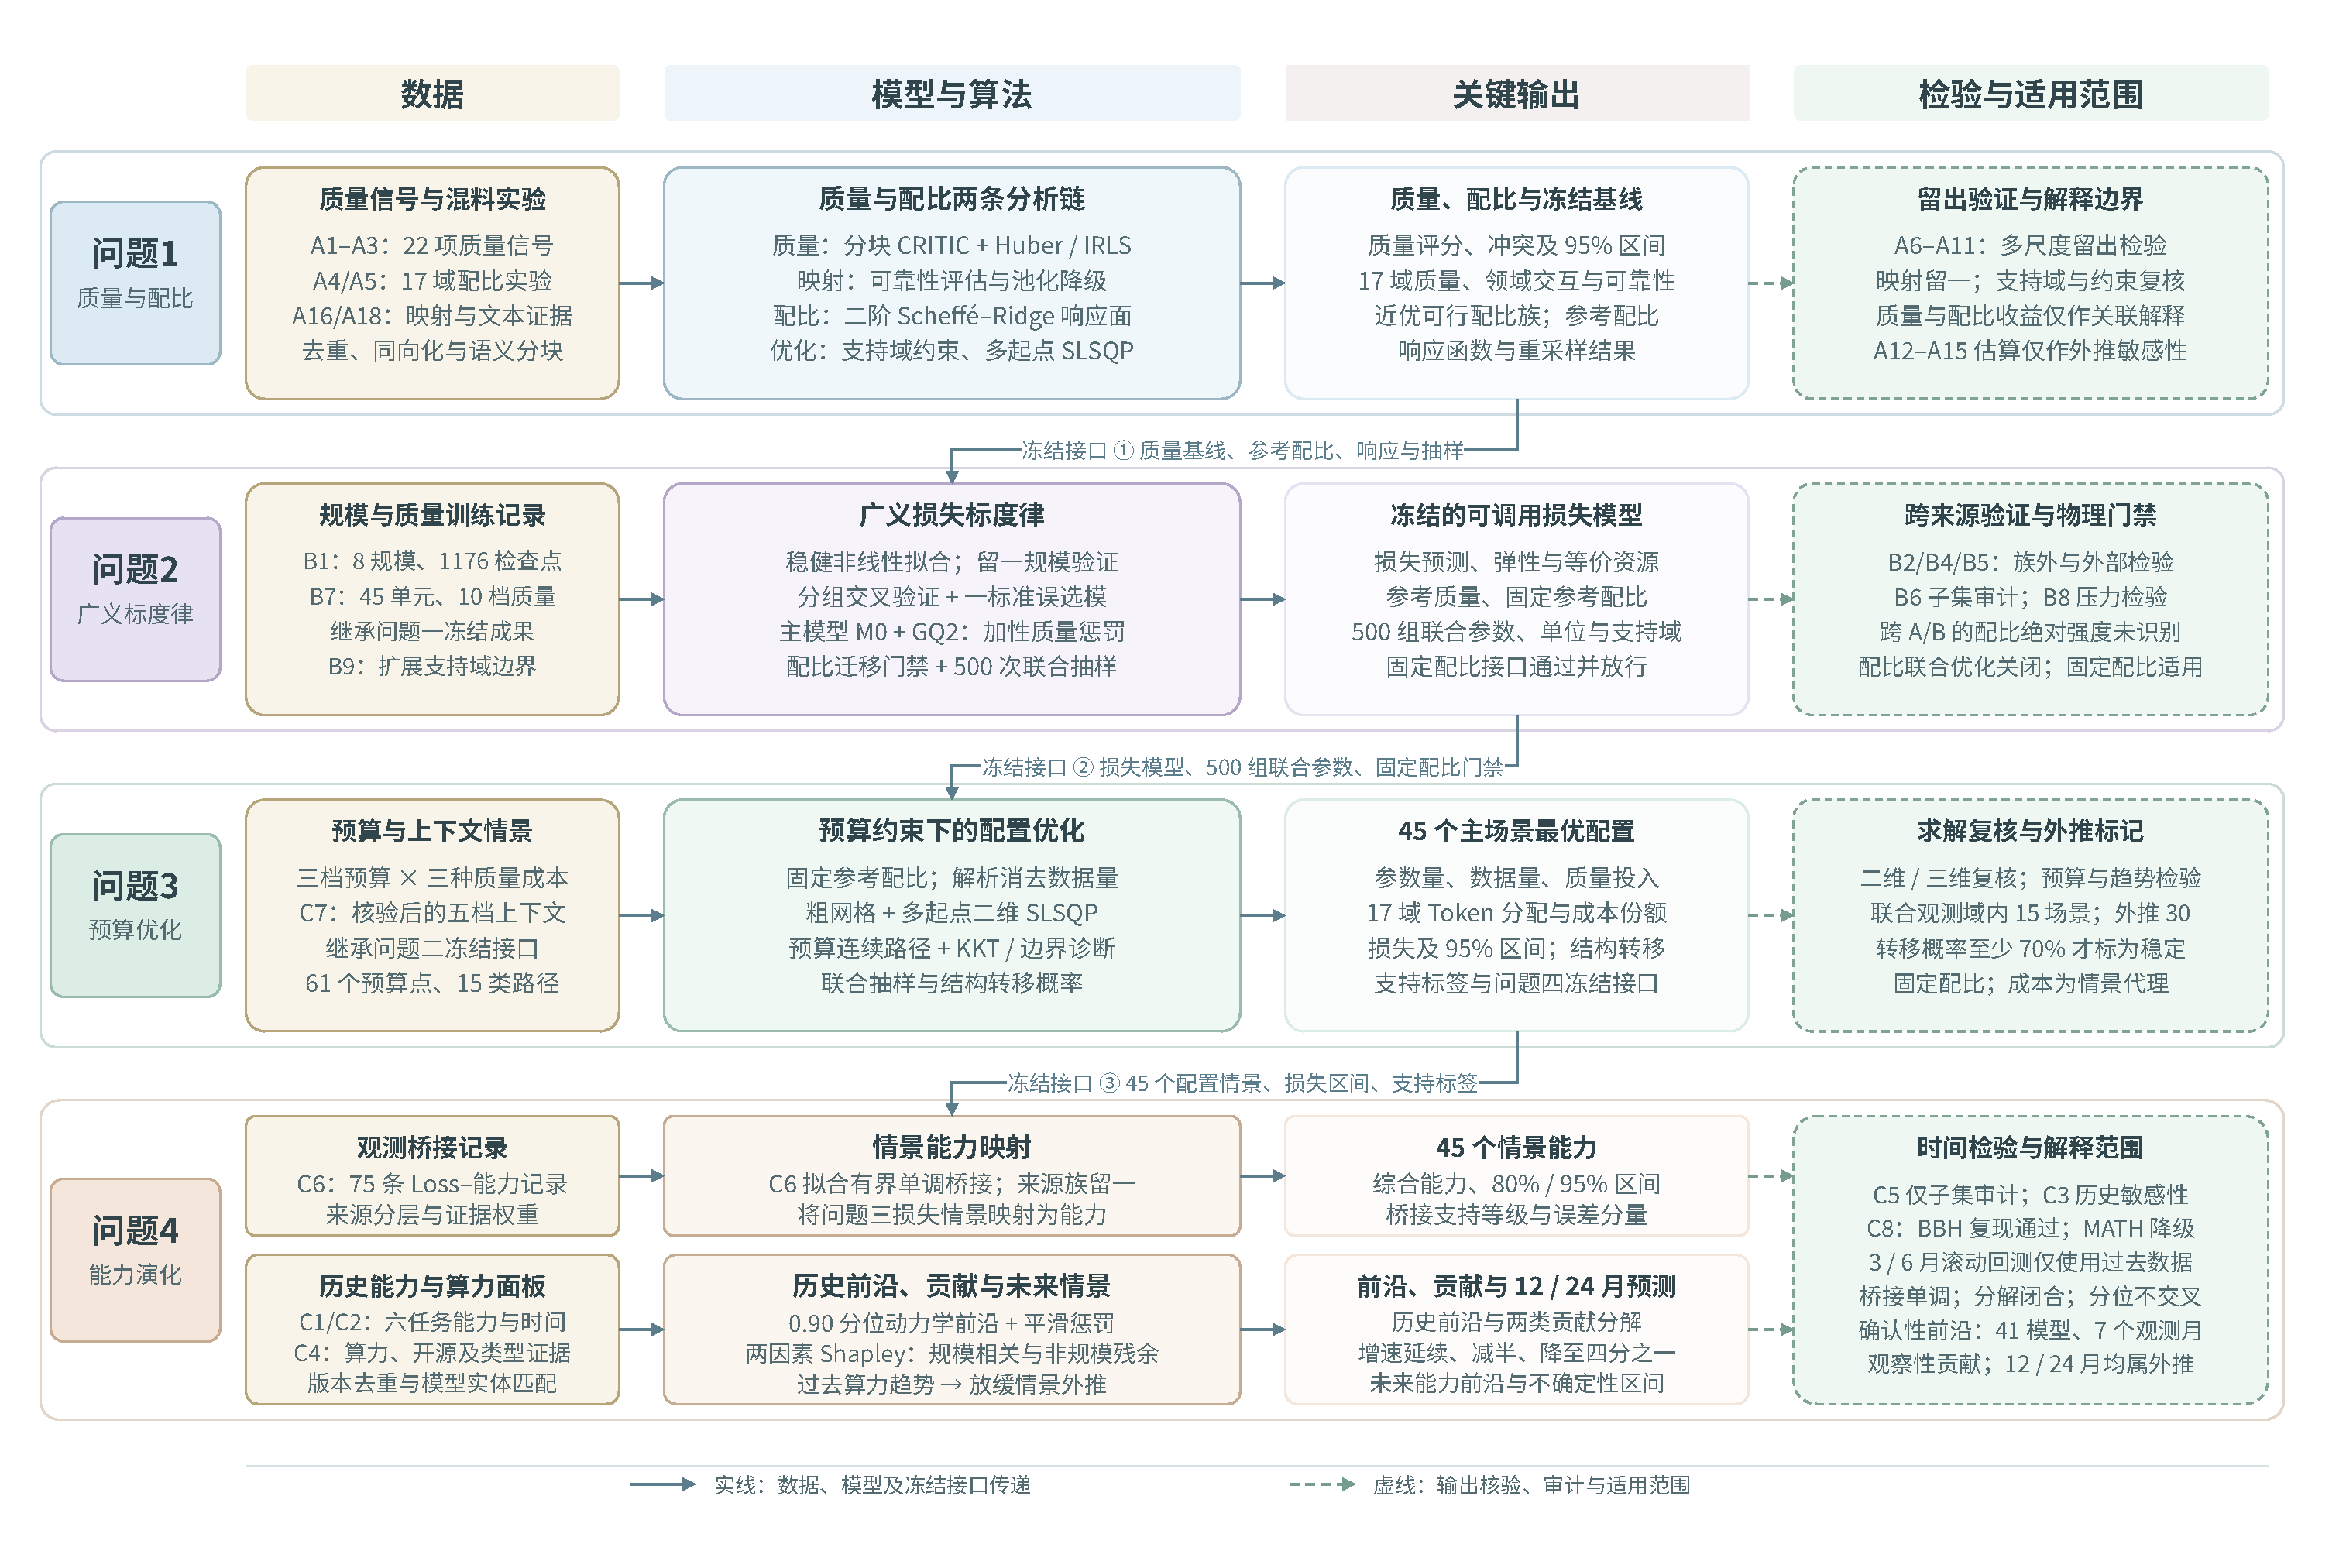
\includegraphics[width=0.98\linewidth]{images/F00_四问关系.pdf}
\caption{四个问题的数据依赖、模型接口与验证关系}
\label{fig:overall_dependency}
\end{figure}

图~\ref{fig:overall_dependency} 中，横向链条表示每一问从数据到模型、输出和检验的内部闭环，纵向连线表示跨问题传递的冻结接口。实线用于模型计算和已验收结果传递，虚线用于跨来源映射、敏感性分析或适用边界检查。特别地，问题一的近优配比 $\boldsymbol p^\star$ 只用于候选方案和方向判断；问题二、三的主链固定 $\boldsymbol p=\boldsymbol p_{\mathrm{ref}}$，从而避免把尚未识别的跨体系配比强度写入中心决策。

\subsection{问题三求解框架}

问题三承接前两问时，先检查冻结标度律、参考配比和上下文证据是否满足接口门槛，再在不同预算、质量成本和上下文情景下求解中心配置；随后沿连续预算路径识别结构转移，并以独立复核、联合抽样和支持域标签完成验收。该过程按“冻结接口--预算优化--路径诊断”分为三层，如图~\ref{fig:p3_overall_framework}所示。

\begin{figure}[H]
\centering
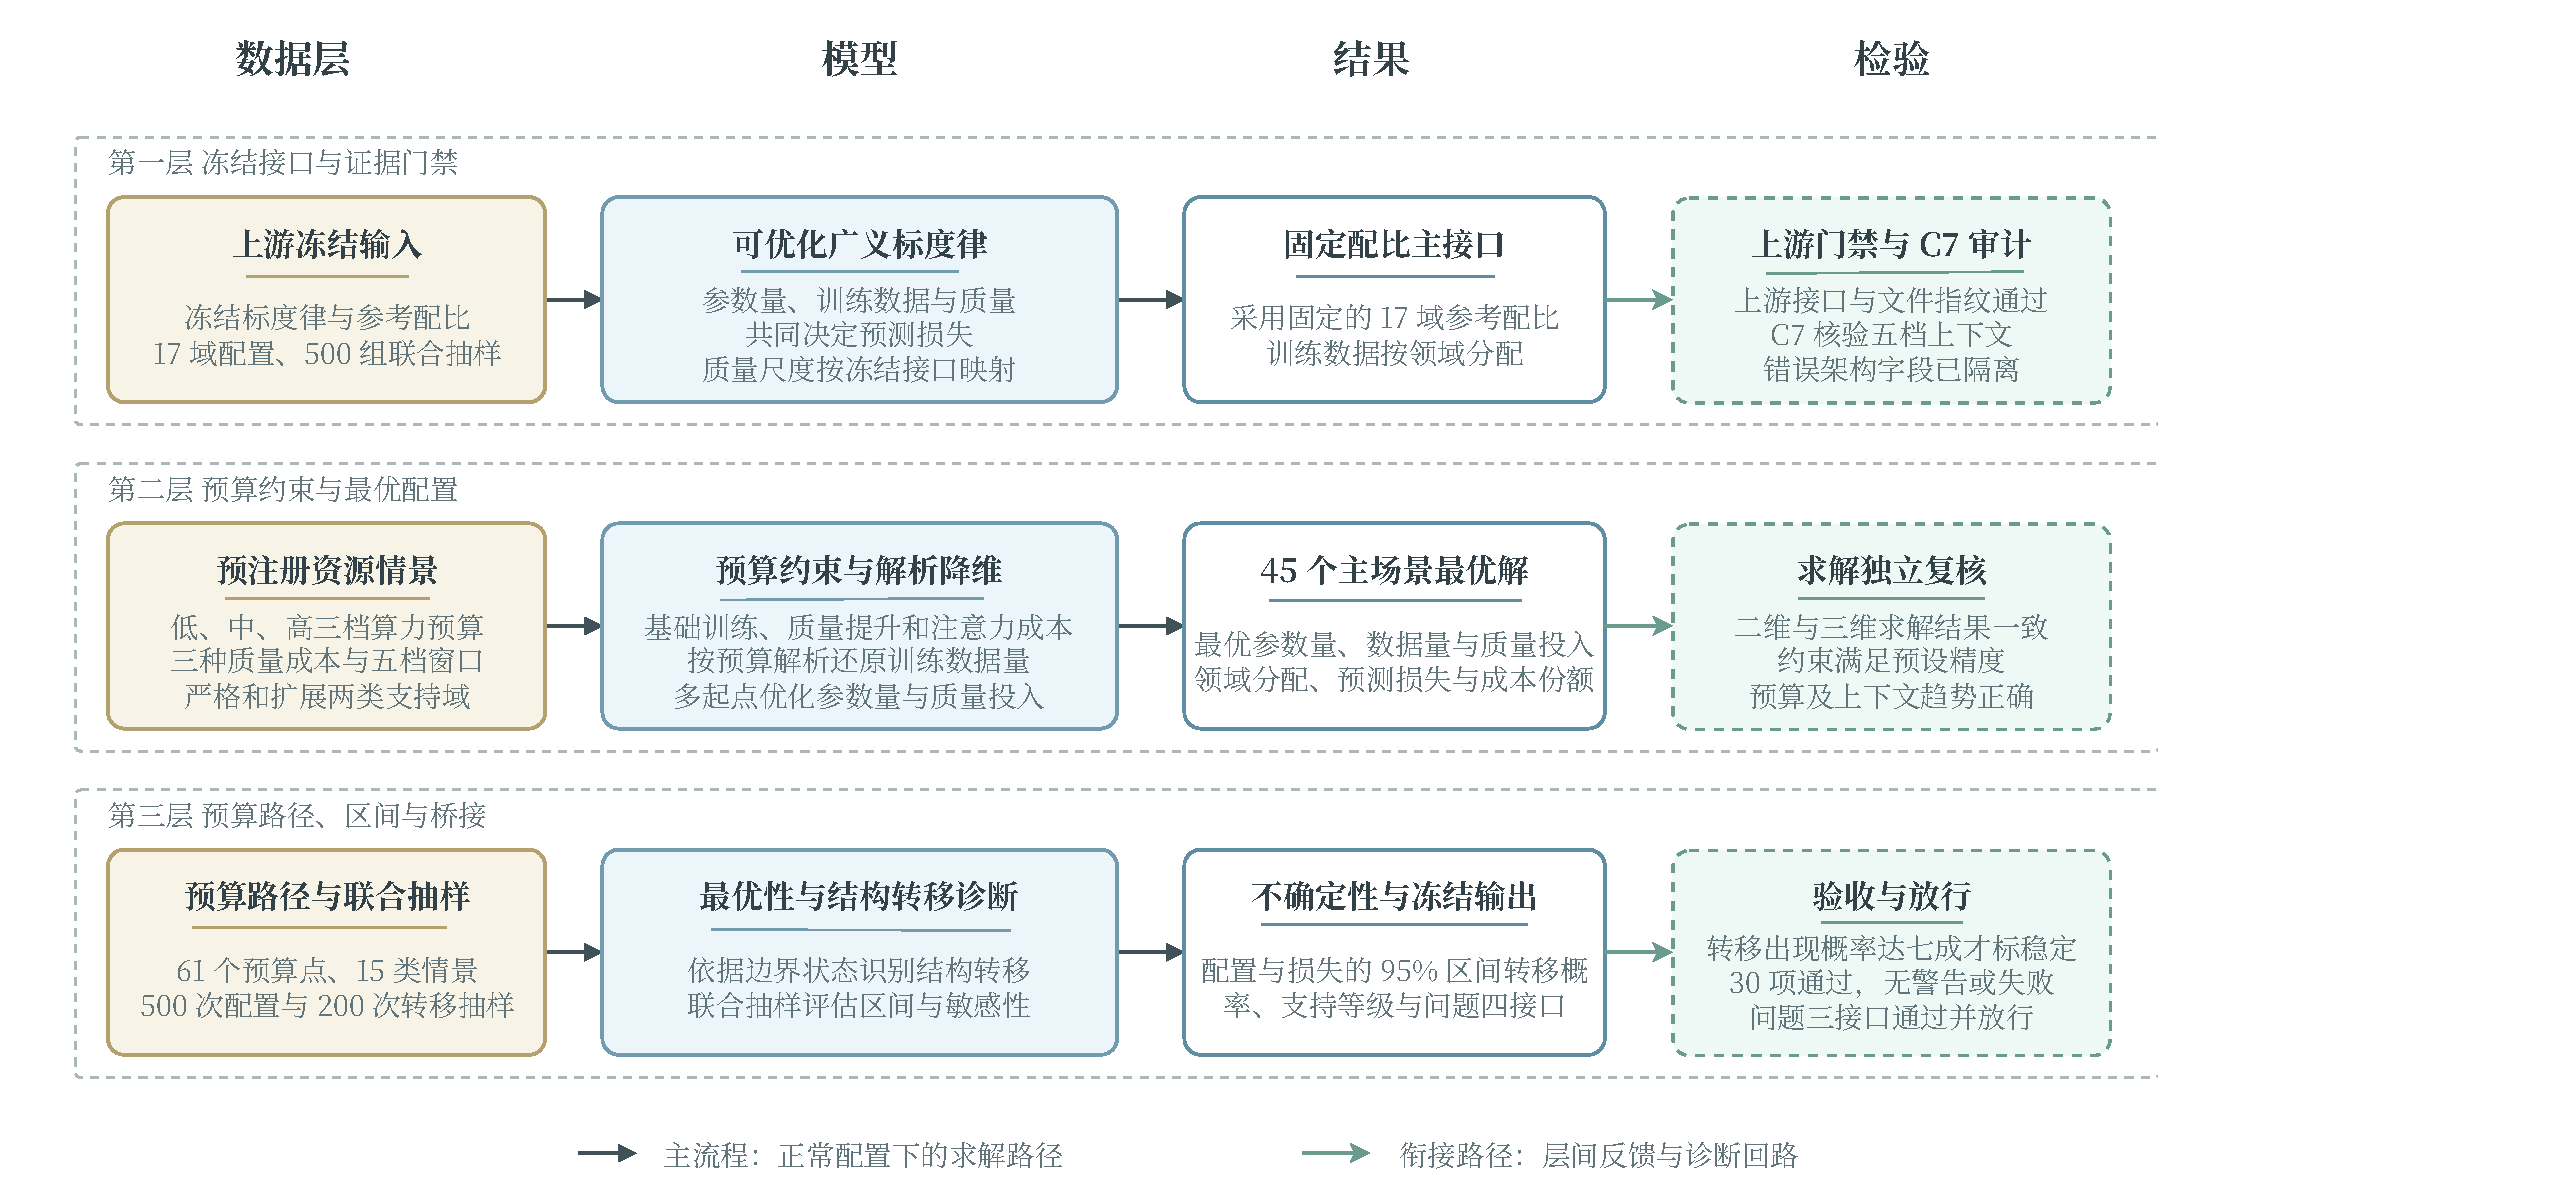
\includegraphics[width=0.98\linewidth]{images/no3/P3_F00R_问题三框架图.pdf}
\caption{问题三从冻结接口到优化验收的分层建模框架}
\label{fig:p3_overall_framework}
\end{figure}

该框架把中心求解与证据审计并列组织：中心链输出参数量、数据量、质量投入和领域 Token 分配，诊断链同时报告约束可行性、求解一致性、结构转移概率与外推等级。由此，问题三输出的不只是一个最优点，而是带有适用范围和不确定性说明的条件最优配置。
